\documentclass[11pt]{article}
\usepackage{acl2014}
\usepackage{times}
\usepackage{url}
\usepackage{latexsym}
\usepackage{booktabs}
\usepackage{multirow}
\usepackage{graphicx}
\usepackage[dvipsnames]{xcolor}
\definecolor{linkcopper}{HTML}{BC6C25}
\usepackage[colorlinks=true, urlcolor=linkcopper, linkcolor=linkcopper, citecolor=linkcopper]{hyperref}
\makeatletter
\def\@biblabel#1{}
\def\citename#1{#1}
\makeatother

\setlength\titlebox{5cm}
\title{
  \LARGE Understory \\[0.4em]
  \large Mapping Natural Agency in Romantic Literature
}

\author{Sara Roggiani \\
    {\tt sara.roggiani2@studio.unibo.it}
}

\begin{document}
\maketitle

\section{Introduction}
Understory investigates the presence and agency of the \textbf{natural world} in literary texts. The grammatical position given to nature – as an active participant or as the object of human action – offers one way of studying how a text imagines the relationship between humans and the natural world.

To explore this relationship, a \textbf{custom fine-tuned BERT model} identifies non-human natural entities across a corpus of English Romantic literature, classifying them into five categories: flora, fauna, weather, landscape, and nature. A \textbf{dependency-based grammatical analysis} then examines the syntactic role each entity occupies within its sentence.

Together, these two stages investigate not only which forms of nature appear in the texts, but also how they participate in their language.


\section{Background and State of the Art}

The idea behind Understory emerged from \textbf{ecocriticism}. In literary studies, it is the approach that examines how texts represent the relationship between human beings and the natural world, based on the premise that language does not merely describe nature but actively shapes how it is perceived \cite{bate:91}. From this perspective, the ways in which nature is represented can reveal the underlying role it plays within a given text.

The \textbf{computational study of entities} and their animacy provides a methodological background for this research. Previous research has explored how entities typically considered inanimate may be linguistically represented as animate. Jahan et al.~\shortcite{Jahan:18} examine animacy beyond the word level, while Coll Ardanuy et al.~\shortcite{collardanuy:20} explore how typically inanimate entities, such as machines, can be represented as animate. Such studies highlight the value of moving beyond conventional distinctions between animate/inanimate entities and of analyzing how linguistic context affects entity representation.

These perspectives are combined with \textbf{Natural Language Processing} (NLP), using Named Entity Recognition (NER) to identify and classify natural entities and dependency analysis to examine their grammatical relationships. Research on the adaptation of language models to specialized and relatively small datasets further demonstrates the applicability of these methods to domain-specific textual material \cite{dodge:20}.

Understory brings these areas together to translate a literary question into a computationally observable one. Rather than replacing close reading, the analysis is conceived as a complementary tool for detecting patterns across large bodies of text.


\section{Data and Methods}
\subsection{Data and Annotation}
The source corpus consists of thirteen passages from five Romantic English authors (Table 1), selected as a historically and culturally situated context in which nature occupies a central role in literary language \cite{bate:91}. The passages were sourced from Project Gutenberg and cleaned to remove non-narrative elements (table of contents, footnotes, headings) before sampling.

\begin{table*}[t]
\centering
\caption{Source corpus}
\label{tab:corpus}
\vspace{4pt}
\begin{tabular}{llr}
\toprule
\textbf{Author} & \textbf{Work} & \textbf{Words} \\
\midrule
Samuel Taylor Coleridge & The Rime of the Ancient Mariner & 3822 \\
\midrule
\multirow{3}{*}{William Wordsworth}
  & Lines Written a Few Miles above Tintern Abbey & 1229 \\
  & Lines Written in Early Spring & 154 \\
  & The Tables Turned & 188 \\
\midrule
\multirow{4}{*}{Percy Shelley}
  & Ode to the West Wind & 4800 \\
  & Mont Blanc & 1092 \\
  & The Cloud & 604 \\
  & To a Skylark & 565 \\
\midrule
\multirow{2}{*}{Mary Shelley}
  & Frankenstein – Letters 1-4 (Arctic frame) & 5512 \\
  & Frankenstein – Chapter 10 (glacier scene) & 2357 \\
\midrule
\multirow{3}{*}{Lord Byron}
  & Childe Harold's Pilgrimage – Canto III & 2507 \\
  & Manfred – Act I, Scene II & 980 \\
  & Manfred – Act II, Scene II & 1513 \\
\bottomrule
\end{tabular}
\end{table*}

Then, candidate sentences were identified using a \textbf{WordNet-derived lexicon} \cite{miller:95} of potentially nature-related terms. Each sentence was assigned a density score, based on the number of candidates it contained, and grouped into four bands (0, 1, 2, 3+). The final sample was stratified across these bands to ensure both sparse and entity-rich sentences were represented. This step was fully automatic and served only to guide sentence sampling; manual annotation began after the 305-sentence sample had been fixed. \\ \\

Since WordNet does not consider context, \textbf{spaCy} part-of-speech tagging restricted candidates to noun mentions, which were then manually verified (particularly for figurative and archaic terms). The \textbf{manual annotation} followed project-specific guidelines developed before and refined during the process. The resulting gold-standard dataset contains 795 entity mentions across five categories: flora, fauna, weather, landscape, and Nature.

\subsection{BERT Fine-Tuning for NER}
A pretrained BERT model \cite{devlin:19} was fine-tuned for token-level classification to identify and classify non-human entities using the annotated dataset. A supervised, span-based approach was chosen because the project requires the model to identify entity spans and assign them to a domain-specific category. Therefore, BERT was fine-tuned using the \textbf{BIO tagging scheme} \cite{ramshaw:95}: each token is labeled B- (beginning), I-(inside), or O (outside an entity), allowing multi-word entities such as \textit{West Wind} to be represented as single spans.

The resulting label set comprises eleven classes: O for non-entity tokens, and B-/I- labels for each of the five categories. Since BERT’s tokenizer may split words into multiple subword units, only the first one receives a label, with subsequent subwords excluded from the loss and evaluation. Before training, the BIO representation was independently validated by decoding labels back into character-level spans and comparing them with the original annotations to catch boundary inconsistencies beforehand.

A central challenge was the strong \textbf{class imbalance} in the annotated data: approximately 95\% of tokens belong to the O class, with entity categories unevenly represented. Class-weighted cross-entropy loss, using inverse-frequency weights, was selected to address this. An initial scheme assigned too little weight to O, producing excessive false positives (precision 0.27, recall 0.87, F1 0.41 on a diagnostic fold); a minimum weight of 0.3 corrected this (precision 0.49, F1 0.61), indicating the weighting needed to balance false positives against false negatives rather than simply emphasize rare classes. This value anchored a systematic sweep through five-fold cross-validation: reducing the maximum weight from 20 to 10 improved performance consistency across folds, and a further reduction to 5 produced additional gains for FAUNA and NATURE; increasing the minimum weight from 0.3 to 0.5 then improved F1 across all folds, while a further increase to 0.7 offered no aggregate improvement. The final configuration (MIN\_WEIGHT = 0.5, MAX\_WEIGHT = 5.0) raised mean F1 from 0.70 to 0.76.

\textbf{Five-fold multilabel stratified cross-validation} was used for evaluation and parameter refinement to distribute rare categories evenly across folds, ensuring NATURE was represented in all five. The model was trained for up to six epochs with early stopping based on validation loss, using a learning rate of 2e-5, batch size of 8, and weight decay of 0.01.

A \textbf{confidence threshold} was introduced as a post-processing step to prioritize precision over recall and reduce low-confidence false positives \cite{zhu:22}. Thresholds between 0.6 and 0.8 produced a broad optimum, with 0.7 selected as the best-supported value (Table 2). This threshold raised the mean F1 to approximately 0.79 through much higher precision with only a limited reduction in recall. However, under this final thresholded configuration, NATURE’s specific F1 fell from 0.58 to 0.24, driven by a sharp drop in recall (see Discussion for a more detailed analysis).

\begin{table}[t]
\centering
\caption{NER Performance Across Confidence Thresholds}
\label{tab:threshold}
\vspace{4pt}
\begin{tabular}{lrrr}
\toprule
\textbf{Threshold} & \textbf{Precision} & \textbf{Recall} & \textbf{F1} \\
\midrule
0.0 & 0.684 & 0.848 & 0.757 \\
0.1 & 0.684 & 0.848 & 0.757 \\
0.2 & 0.686 & 0.848 & 0.758 \\
0.3 & 0.693 & 0.845 & 0.762 \\
0.4 & 0.717 & 0.841 & 0.774 \\
0.5 & 0.748 & 0.829 & 0.786 \\
0.6 & 0.771 & 0.809 & 0.789 \\
\textbf{0.7} & \textbf{0.799} & \textbf{0.787} & \textbf{0.793} \\
0.8 & 0.828 & 0.751 & 0.788 \\
0.9 & 0.884 & 0.658 & 0.754 \\
\bottomrule
\end{tabular}
\end{table}

Finally, the model’s predictions were examined \textbf{qualitatively}, both to identify recurring error patterns and to complement the quantitative evaluation by indicating where and why the model struggled. These included generic uses of \textit{nature}, human/animal confusion, and complex or hyphenated multi-word. The errors largely occurred around the same semantic and linguistic boundaries that had proved difficult during manual annotation, suggesting that the model’s limitations are closely connected to the interpretive complexity of the corpus.

The final model was retrained on the complete annotated dataset using the final configuration and run on the remaining unannotated sentences.


\subsection{Dependency-Based Grammatical Role Analysis}
The identified entities were then analyzed through dependency parsing to investigate natural agency, defined here in grammatical rather than theoretical terms. Active subjects are treated as agentive, while passive subjects, direct objects, and objects of prepositions represent progressively less agentive roles.

The entities were passed through spaCy. The transformer-based model \texttt{en\_core\_web\_trf} was chosen over \texttt{en\_core\_web\_sm} because of the corpus’s frequent archaic constructions and inverted word order. \textbf{Parser reliability} was assessed comparing the two models directly. Among 20 manually adjudicated disagreements, the transformer model was correct in 14 cases (70\%), compared with 2 (10\%) for the smaller model. This was treated as evidence of relative suitability rather than perfect parser accuracy.

The resulting dataset pairs each natural entity with its category and grammatical role.

\begin{figure*}[t]
\centering
\caption{Grammatical Role by Entity Type}
\makeatletter
\renewcommand{\@makecaption}[2]{\centering #1\par}
\makeatother
\label{fig:role_by_genre}
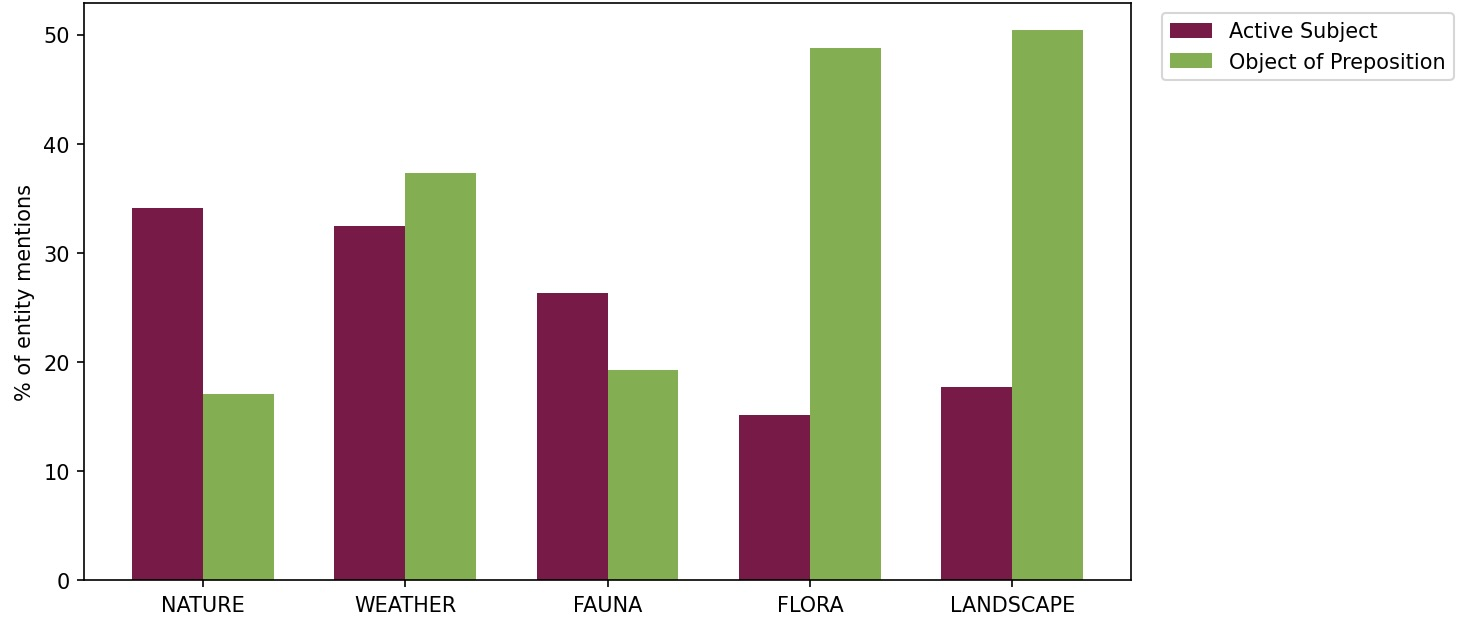
\includegraphics[width=0.85\textwidth]{figure1.jpeg}
\end{figure*}


\subsection{LLM Comparison}
The Romantic corpus was treated as a historically situated case study, raising the question of whether its grammatical patterns are specific to Romantic writing or observable more broadly. Since collecting and annotating comparable corpora was beyond the project’s scope, large language model (LLM) generation was used to create text across different literary traditions, processed through the same pipeline already described.

This comparison needs a reminder: the LLM instructed to write in a given style does not reproduce that tradition directly but generates text from its own learned representation of it, which may be partial or biased. Results are therefore treated as an indication of how the model responds to genre prompts, not as literary evidence about the genres themselves.

Text was generated using the \textbf{Gemini API} \texttt{gemini-3.6-flash}). Its free-tier limit of twenty requests per day determined the experimental design: five literary conditions $\times$ four topics, yielding twenty passages of 150-200 words each. Each scenario is generic so that any natural entities in the generated text would emerge from each genre’s own conventions rather than being guaranteed by the prompt. After processing through the same pipeline, 146 natural entity mentions were identified.

A narrower comparison then examined the English Romanticism condition against the original corpus, comparing entity-category composition and grammatical-role distribution to assess whether the generated texts reproduce its grammatical patterns rather than merely its vocabulary and imagery.

\section{Results}

\subsection{Grammatical Role by Entity Type}
The most notable result (Figure 1) is that NATURE showed the highest proportion of active-subject positioning, at 34.1\% narrowly exceeding WEATHER (32.5\%). LANDSCAPE and FLORA showed the opposite tendency: objects of prepositions accounted for 50.4\% and 48.8\% respectively, compared with only 17.7\% and 15.1\% as active subjects.

The \textbf{convergence between semantic definition and syntactic behavior} is particularly notable because the two were derived entirely independently: the categories through human annotation and the grammatical roles through automated dependency parsing. The categories themselves were never defined with reference to agency or grammatical structure, yet the resulting distribution appears to track the conceptual distinction established during annotation.

\subsection{LLM Analysis}
The cross-genre comparison showed substantial variance in entity density. English Romanticism produced 13.25 natural entities per passage, compared to 5.25-7.00 in other conditions despite identical prompts. NATURE appeared exclusively in the English Romanticism texts, while WEATHER and LANDSCAPE were present across all five (Table 3). Grammatical-role distributions also differed: Russian Literature had the highest active-subject rate (27.3\%), while American Dystopian fiction had the lowest (9.1\%).

The comparison with generated English Romanticism texts and the original corpus showed that WEATHER was more frequent in the generated texts (56.6\% vs. 41.7\%), while LANDSCAPE was less frequent (26.4\% vs. 38.8\%). FLORA and WEATHER showed broadly comparable grammatical distributions, whereas LANDSCAPE was much more concentrated in prepositional roles in the generated texts (78.6\% vs. 50.4\%). NATURE and FAUNA were too sparse for meaningful comparison.


\begin{table*}[t]
\centering
\caption{Entity category composition by genre}
\label{tab:genre_composition}
\vspace{4pt}
\begin{tabular}{lrrrrrr}
\toprule
\textbf{Genre} & \textbf{FLORA} & \textbf{FAUNA} & \textbf{WEATHER} & \textbf{LANDSCAPE} & \textbf{NATURE} & \textbf{Total (n)} \\
\midrule
English Romanticism & 15\% & 0\% & 57\% & 26\% & 2\% & 53 \\
American Dystopian  & 9\%  & 5\% & 64\% & 23\% & 0\% & 22 \\
Russian Literature  & 9\%  & 0\% & 73\% & 18\% & 0\% & 22 \\
Historical Romance  & 4\%  & 4\% & 75\% & 18\% & 0\% & 28 \\
British Fiction     & 19\% & 0\% & 57\% & 24\% & 0\% & 21 \\
\bottomrule
\end{tabular}
\end{table*}


\section{Web Application}
To make the entire analysis usable beyond the research corpus, the pipeline was implemented as Flask web application, allowing users to parse or upload text and run the same NER and dependency analysis.

Because BERT accepts a maximum of 512 tokens, longer texts are divided into sentence-aligned chunks using spaCy boundaries, preventing entities from being split across chunks. The interface presents predictions directly within the submitted text, highlighting entities by category, alongside a table listing each entity’s category and grammatical role.

\section{Discussion}
The central findings – the convergence between semantic definition and syntactic behavior and the particularly high rate of active-subject positioning for NATURE – provide a syntactic perspective on an established ecocritical observation: Romantic poetry can represent nature as capable of independent action rather than merely as a passive background \cite{bate:91}. Since NATURE was defined during annotation solely on semantic grounds, independently of grammatical structure, this convergence cannot be attributed to a circular definition.

Several \textbf{limitations} should be considered when interpreting these findings. First, \textbf{NATURE} is the least reliably recognized category in the final model: its F1 falls from 0.58 to 0.24 after thresholding. This suggests the model’s confidence scores were not a reliable correctness signal for this category. The 34.1\% active-subject rate should therefore be read as indicative rather than precise, resting on the project’s smallest and least stable category.

Second, annotation was performed by a \textbf{single annotator}, preventing calculation of inter-annotator agreement. Third, the corpus is strongly weighted towards \textbf{poetry} (eleven of thirteen passages), whose inversion, ellipsis, and compressed syntax create particular difficulties for dependency parsing. Finally, the \textbf{small dataset} prevented the use of a fully independent test set, although k-fold cross-validation provided a practical solution for this low-resource setting.

Despite the limitations, the project demonstrates how a literary question can be translated into a computationally observable pattern, examining not only which forms of nature appear in a text but how they are positioned within its language.

\section{Future Developments}
\textbf{Category-specific confidence threshold.} As discussed in Section 6, the global threshold disproportionately reduced NATURE’s recall and precision; a lower, category-specific threshold could recover this without affecting the gains elsewhere. This would require retraining and re-analysis of the full pipeline. \\

\textbf{Figurative column.} The annotation schema includes a \texttt{is\_figurative} column, that could be cross-referenced against grammatical role to test whether metaphorically-invoked entities are positioned differently than literal ones.

\textbf{A masked-prediction diagnostic.} Coll Ardanuy et al.~\shortcite{collardanuy:20} use masked-word prediction to probe contextual expectations around animacy; applying this to already-identified entities could offer a complementary perspective, independent of the supervised approach used here.

\newpage
\onecolumn

\begin{thebibliography}{}

\bibitem[\protect\citename{Bate}1991]{bate:91}
J. Bate.
\newblock 1991.
\newblock Romantic Ecology: Wordsworth and the Environmental Tradition.
\newblock Routledge, London.

\bibitem[\protect\citename{Coll Ardanuy \bgroup et al.\egroup}2020]{collardanuy:20}
M. Coll Ardanuy, F. Nanni, K. Beelen, K. Hosseini, R. Ahnert, J. Lawrence, K. McDonough, G. Tolfo, D. CS Wilson, and B. McGillivray.
\newblock 2020.
\newblock \href{https://aclanthology.org/2020.coling-main.400/}{Living Machines: A study of atypical animacy}.
\newblock In {\em Proceedings of the 28th International Conference on Computational Linguistics}, pages 4534--4545, Barcelona, Spain (Online). International Committee on Computational Linguistics.

\bibitem[\protect\citename{Devlin \bgroup et al.\egroup}2019]{devlin:19}
J. Devlin, M.-W. Chang, K. Lee, and K. Toutanova.
\newblock 2019.
\newblock \href{https://aclanthology.org/N19-1423/}{BERT: Pre-training of Deep Bidirectional Transformers for Language Understanding}.
\newblock In {\em Proceedings of the 2019 Conference of the North American Chapter of the Association for Computational Linguistics: Human Language Technologies, Volume 1 (Long and Short Papers)}, pages 4171–4186, Minneapolis, Minnesota. Association for Computational Linguistics.

\bibitem[\protect\citename{Dodge \bgroup et al.\egroup}2020]{dodge:20}
J. Dodge, G. Ilharco, R. Schwartz, A. Farhadi, H. Hajishirzi, and N. A. Smith.
\newblock 2020.
\newblock Fine-Tuning Pretrained Language Models: Weight Initializations, Data Orders, and Early Stopping.
\newblock arXiv:2002.06305.

\bibitem[\protect\citename{Jahan \bgroup et al.\egroup}2018]{Jahan:18}
L. Jahan, G. Chauhan, and M. Finlayson.
\newblock 2018.
\newblock \href{https://aclanthology.org/C18-1001/}{A New Approach to Animacy Detection}.
\newblock In {\em Proceedings of the 27th International Conference on Computational Linguistics}, pages 1-12, Santa Fe, New Mexico, USA. Association for Computational Linguistics.

\bibitem[\protect\citename{Miller}1995]{miller:95}
G. A. Miller.
\newblock 1995.
\newblock \href{https://aclanthology.org/H92-1116/}{WordNet: A Lexical Database for English}.
\newblock {\em In Speech and Natural Language: Proceedings of a Workshop Held at Harriman, New York, February 23-26, 1992}.

\bibitem[\protect\citename{Ramshaw and Marcus}1995]{ramshaw:95}
L. A. Ramshaw and M. P. Marcus.
\newblock 1995.
\newblock \href{https://aclanthology.org/W95-0107/}{Text Chunking Using Transformation-Based Learning}.
\newblock In {\em Third Workshop on Very Large Corpora}.

\bibitem[\protect\citename{Zhu and Li}2022]{zhu:22}
E. Zhu and J. Li.
\newblock 2022.
\newblock \href{https://aclanthology.org/2022.acl-long.490/}{Boundary Smoothing for Named Entity Recognition}.
\newblock In {\em Proceedings of the 60th Annual Meeting of the Association for Computational Linguistics (Volume 1: Long Papers)}, pages 7096–7108, Dublin, Ireland. Association for Computational Linguistics.

\end{thebibliography}

\vspace{20pt}

\appendix
\section*{Index of Outputs}
All the material produced is available on the
\href{https://github.com/sararoggi/understory}{GitHub repository}.

\begin{center}
\vspace{4pt}
\begin{tabular}{llr}
\toprule
\textbf{Path} & \textbf{Description} \\
\midrule
 \texttt{data/corpus/} & Corpus data \\
\midrule
 \texttt{data/annotations/final\_annotation.csv} & Gold-standard annotated dataset \\
\midrule
 \texttt{data/model\_evaluation/} & NER model evaluation results \\
\midrule
 \texttt{data/model\_predictions/} & NER model predictions \\
\midrule
 \texttt{data/dependency\_analysis/} & Dependency analysis results  \\
\midrule
 \texttt{data/llm\_texts/} & LLM-generated texts and analysis results  \\
\midrule
 \texttt{notebooks/setup.ipynb} & Corpus construction and resource caching  \\
\midrule
 \texttt{notebooks/annotation.ipynb} & WordNet-based candidate selection for annotation  \\
\midrule
 \texttt{notebooks/ner\_model.ipynb} & BERT fine-tuning, evaluation, and inference  \\
\midrule
 \texttt{notebooks/dependency\_analysis.ipynb} & Dependency analysis  \\
\midrule
 \texttt{notebooks/llm\_analysis.ipynb} & LLM-based comparative analysis  \\
\midrule
 \texttt{docs/annotation\_guidelines.md} & Annotation guidelines  \\
\midrule
 \texttt{app/} & Flask web application  \\
\bottomrule
\end{tabular}
\end{center}

\end{document}